% !TeX encoding = UTF-8
% !TeX program = pdfLaTeX
% !TeX root = matlab-exercises-emaip.tex
% !TEX bibfile = file.bib
% !TeX spellcheck = en_GB
\documentclass[12pt,a4paper]{article}
\usepackage[colorlinks, linkcolor=blue, citecolor=blue, urlcolor=blue]{hyperref}
%\usepackage[nosolutionfiles]{answers}
\usepackage{answers}
\usepackage{graphicx}
\usepackage{amsmath}
\usepackage{todonotes}
\usepackage{listings}
\usepackage{color}
\definecolor{dkgreen}{rgb}{0,0.6,0}
\definecolor{gray}{rgb}{0.5,0.5,0.5}

\lstset{language=Matlab,
   keywords={break,case,catch,continue,else,elseif,end,for,function,
      global,if,otherwise,persistent,return,switch,try,while},
   basicstyle=\footnotesize\ttfamily,
   keywordstyle=\color{blue},
   commentstyle=\color{dkgreen},
   stringstyle=\color{dkgreen},
%   numbers=left,
%   numberstyle=\tiny\color{gray},
%   stepnumber=3,
%   numbersep=10pt,
   backgroundcolor=\color{white},
   tabsize=4,
   showspaces=false,
   showstringspaces=false}

\newcommand{\moved}{\todo[inline]{The exercise above has been moved to matlab with unittests.}}


% Fix for moving the hypertarget one line up.
% https://tex.stackexchange.com/a/412381/1366
\makeatletter
 \newcommand{\linkdest}[1]{\Hy@raisedlink{\hypertarget{#1}{}}}
\makeatother

\newcounter{ex}
\numberwithin{ex}{section}

\newenvironment{ex}[1][]{%
\filbreak
\bigskip
\refstepcounter{ex}
\noindent
\textbf{\linkdest{\theex{}exercise}{}Exercise \theex{}: #1\hfill\hyperlink{\theex{}hint}{hint}, \hyperlink{\theex{}solution}{solution}}\par\noindent}{}

\Newassociation{sol}{Solution}{ans}
\Newassociation{hint}{Hint}{hnt}


% Redefine the Hint and Solution environment.
\renewenvironment{Hint}[1]{{\filbreak\par\noindent\linkdest{#1{}hint}{}\bf Exercise \hyperlink{#1{}exercise}{#1}:}\newline}{\bigskip}
\renewenvironment{Solution}[1]{{\filbreak\par\noindent\linkdest{#1{}solution}{}\bf Exercise \hyperlink{#1{}exercise}{#1}:}\newline}{\bigskip}

\Opensolutionfile{ans}[ans]
\Opensolutionfile{hnt}[hints]

\author{Henrik Skov Midtiby}
\title{Matlab exercises for E-MAIP 2019}
\date{\today}


\begin{document}
\maketitle

\newpage
\tableofcontents

\newpage
\section*{Introduction}

These notes are used in the course \emph{Mathematics and Introduction to programming}
that is taught on University of Southern Denmark during fall 2019.

The source for this document is available on github, 
\url{https://github.com/henrikmidtiby/matlab-notes}.



\section{Setting git up on Windows}

In this section it is explained how to set up git on 
a Windows computer.
This is also described in this \href{https://tekvideo.sdu.dk/t/henrikmidtiby/E-MAIP-2020/2020/1/blok04/4}{video}.

The steps are as follows:
\begin{enumerate}
\item		Download and install \emph{Git for Windows} from \url{https://git-scm.com/}
\item		Open \emph{Git Bash} and identify yourself to git
\item		Generate an ssh key
\item 	Add the generated ssh key to \url{https://gitlab.sdu.dk}
\end{enumerate}

\subsection{Download and installation of \emph{Git for Windows}}

Open \url{https://git-scm.com/} and click on the download button
in the right side of the page.

\subsection{Open Git Bash and identify yourself to git}

Find the \emph{Git Bash} program and start it.
It will look like a black image with some coloured text in the 
top left corner.
What is opened now is a computer console or terminal.
It can be very effective to do certain tasks on the computer through the console.

To set name and email that the git installation uses on the 
computer, the following commands should be executed:
\begin{verbatim}
git config --global user.name "<your name>"
git config --global user.email "<your email>"
\end{verbatim}

For me it looked like this:
\begin{verbatim}
hemi@TEK-CB-HEMI-01 MINGW64 ~
$ git config --global user.name "Henrik Skov Midtiby"

hemi@TEK-CB-HEMI-01 MINGW64 ~
$ git config --global user.email "hemi@mmmi.sdu.dk"
\end{verbatim}

\subsection{Generate an ssh key}

To work efficiently with git on remote servers like \url{https://gitlab.sdu.dk} or \url{https://github.com}, you need to generate 
an ssh key.
In Git Bash it is done with the command.
\begin{verbatim}
ssh-keygen -t rsa
\end{verbatim}
After executing the command, the \emph{ssh-keygen} program
will ask you a few questions and then the ssh key is generated.
It is appropriate to use the default values, so you can just 
press enter to accept the default values.

On my computer the key generation process looked like this:
\begin{verbatim}
hemi@TEK-CB-HEMI-01 MINGW64 ~
$ ssh-keygen -t rsa
Generating public/private rsa key pair.
Enter file in which to save the key (/c/Users/hemi/.ssh/id_rsa):
Enter passphrase (empty for no passphrase):
Enter same passphrase again:
Your identification has been saved in /c/Users/hemi/.ssh/id_rsa
Your public key has been saved in /c/Users/hemi/.ssh/id_rsa.pub
The key fingerprint is:
SHA256:GBdcG4YGzNMGF9bOZ5oK7P+m+IxO1+8hYpT2g3g/+Ok hemi@TEK-CB-HEMI-01
The key's randomart image is:
+---[RSA 3072]----+
|     oo===+      |
|      +o*o.o     |
|      .+.o.      |
|       + .o o    |
|     .. S  =     |
|      o+ +o      |
|     .o.*o= .    |
|     ..Booo= .   |
|     .+o=*Eoo    |
+----[SHA256]-----+
\end{verbatim}

\subsection{Add ssh key to gitlab.sdu.dk}

As you have now generated an ssh key, you need to locate the 
public part of the key and add that to \url{https://gitlab.sdu.dk}.
This can be done with the following command.
\begin{verbatim}
cat <path to public key>
\end{verbatim}

On my computer the key is placed in this location 
\verb!/c/Users/hemi/.ssh/id_rsa.pub!, which was displayed 
in the output from the key generation step.

\begin{verbatim}
hemi@TEK-CB-HEMI-01 MINGW64 ~
$ cat /c/Users/hemi/.ssh/id_rsa.pub
ssh-rsa AAAAB3NzaC1yc2EAAAADAQABAAABgQCz0X6DyHeyiqcPe8Y+zeQ60Y
4F0sxR2MqNlsL52ZrllRd0toAFvPvmrz9/rT13eHoD+xSIQ5kL44GTZqn9fRmC
lG3ttc1v7Qd/KmAmM5eOpr+cH/c/IbfFGQyiRV7lRz5KES8TFUEs8YNLfLwdHU
cEhmn7x4Zmc7aahTQFTH55EqOt6HU5YoF4vMe0LG+WnhNrh/kwiKN1ndqasEC6
wE3D6K2/Z21j8FcFqvR0PWDubUABQdMN5+huQ7/O7SAVQCeZBYoG2fcn9HRu39
IS8kKQ3AmmrDFUitaWhIWZ+msfmTqJCplYXVlGrlvjcbIVPIgCr/4IL6soWE1V
KL1cEVGV2lAktMqP9cU1E6rYMFMtYIIyjSkE5l2YJZ++A+dgayHOqBx5qPXRq2
k2gRAz8auiV0ztOCRtA09IhzvlH0ZHU126ZoxC72BJpMP6+Rp3r8EJ4LlU2IaI
SXnoSAqXtc8HvngXm74TQpneLSDy+nMKZJ1jpL9dqxtWUM3DbhPyzaM= hemi@
TEK-CB-HEMI-01
\end{verbatim}




\section{2019-09-09 Matlab introduction}
\todo[inline]{Add Matlab introduction exercises}
\todo[inline]{Add exercises about systems of linear equations}


\subsection{Plot of functions}

\begin{ex}
Plot the function $f(x) = cos(x) + 3*sin(3*x)$
over the $x$ range $[-2, 2]$.
Use the following template 
\begin{lstlisting}
% Create evenly distributed x values that covers the range
x = linspace(0, 10, 100);

% Calculate the associated y value
y = sin(x);

% Open a figure and plot the associated x and y values
figure(1);
plot(x, y);
\end{lstlisting}
\begin{hint}
\end{hint}
\begin{sol}
A solution is:
\begin{lstlisting}
% Create evenly distributed x values that covers the range
x = linspace(-2, 2, 100);

% Calculate the associated y value
y = cos(x) + 3*sin(3*x);

% Open a figure and plot the associated x and y values
figure(1);
plot(x, y);
\end{lstlisting}
\end{sol}
\end{ex}



\begin{ex}
Plot the function $f(x) = 1 / (1.1 + sin(4*x))$
over the interval $x \in [-3, 3]$.
\begin{hint}
\end{hint}
\begin{sol}
A solution is:
\begin{lstlisting}
% Create evenly distributed x values that covers the range
x = linspace(-3, 3, 100);

% Calculate the associated y value
y = 1 ./ (1.1 + sin(4*x));

% Open a figure and plot the associated x and y values
figure(1);
plot(x, y);
\end{lstlisting}
\end{sol}
\end{ex}


\subsection{Plot of secant lines}

\begin{ex}
Draw multiple secant lines on the same figure.
The distance between the points that define the secant line
should be reduced before plotting the next secant line.
Use the following distances between the $x$ values:
$h \in {0.2, 0.1, 0.05, 0.02, 0.01}$.
Please use the template below
\begin{lstlisting}
% Create x values
x = linspace(-3, 6, 100);

% Create a function handle for the function to plot.
fh = @(x) 2*x.^2 - x + 1;

% Find the two end points of the secant to plot.
h = 2;
x0 = 0.2;
x1 = x0 + h;
y0 = fh(x0);
y1 = fh(x1);

% Open a figure and plot the x and y values.
figure(2);
hold off;
% Plot the function
plot(x, fh(x));
hold on;
plot([x0, x1], [y0, y1], 'o-');
\end{lstlisting}
\begin{hint}
\end{hint}
\begin{sol}
A solution is:
\begin{lstlisting}
\end{lstlisting}
\end{sol}
\end{ex}

%
%%% Indskrive vektorer og matricer
%A = [1, 2, 3; 2, 3, 1; 1, 1, 1]
%B = [1, 1, 1; 1, 2, 4; 7, 6, 5]
%C = [1; 2; 3]
%
%
%%% Addition
%disp('addition');
%A + A
%A + B
%B + A
%B + B
%
%
%%% Multiplikation
%disp('multiplikation');
%A * A
%A * B
%B * A
%B * B
%
%
%%% 
%% Transponering
%A
%transpose(A)
%A'
%
%
%%% Opgave
%% Find nogle opgaver med matricer og vektorer.
%% Tjek jeres resultater ved at få Matlab til at udføre de samme beregninger
%% som I har gjort i hånden.
%
%
%
%%%
%% Løsning af lineære ligningssystemer
%
%% Givet ligningerne
%% 2*x1 + 5*x2 = 2 og -4*x1+3*x2 = -30.
%% Kan koefficient matricen A og værdi vektoren b opskrives.
%A = [2, 5; -4, 3];
%b = [2; -30];
%
%% Ud fra værdi vektoren og koefficient matricen, kan 
%% løsningen til ligningssystemet bestemmes på følgende 
%% tre forskellige måder.
%A \ b
%inv(A) * b
%linsolve(A, b)
%
%
%%%
%% Opgave
%% Plot ligningerne x + 2y = 3 og 2x - y = 2 i det samme 
%% koordinatsystem.
%% Opskriv ligningsystemet på matrix form og løs det via 
%% linsolve eller lign.
%% Plot løsningen sammen med de to ligninger.
%% Tjek i hånden at det fremkomne resultat løser de oprindelige 
%% ligninger.
%% teknik.
%
%
%
%
%%%
%% Opgave
%% Der er en fejl i den gauss elimination der fremgår herunder.
%% Benyt funktionen rref (reduced row echelon form), til at 
%% finde fejlen, ved at anvende rref på de forskellige delresultater.
%[1, 2, 3, 1; 3, 2, 1, 1; 1, 1, 2, 1]
%[1, 2, 3, 1; 0, -4, -8, -2; 0, -1, -1, 0]
%[1, 2, 3, 1; 0, 1, -2, 0.5; 0, -2, -1, 0]
%[1, 2, 3, 1; 0, 1, -2, 0.5; 0, 0, -5, 1]

%
%\subsection{Compare derivatives}
%
%\begin{ex}
%\begin{lstlisting}
%%% Sammenlign funktion og dens afledte
%x = linspace(-0.5, 6.2, 100);
%fh = @(x) sin(x);
%fh_prime = @(x) cos(x);
%
%figure(3);
%hold off;
%plot(x, fh(x));
%hold on;
%plot(x, fh_prime(x), 'r');
%legend("f(x)", "f'(x)")
%title("Symbolsk afledte")
%
%
%%% Numerisk estimering af afledte
%% Definer x vaerdier funktionen skal plottes for
%x = linspace(-0.5, 6.2, 100);
%dx = 0.001;
%xprime = x + dx;
%
%% Beregn y vaerdier som skal plottes
%fh = @(x) sin(x);
%y = fh(x);
%yprime = sin(xprime);
%dy = yprime - y;
%derivative = dy / dx;
%
%% Aabn en figur og plot x og y vaerdierne.
%figure(2);
%plot(x, fh(x));
%% Hold fast i det der allerede er plottet.
%hold on;
%plot(x, derivative);
%hold off;
%legend("f(x)", "f'(x)")
%title("Numerisk afledte")
%
%
%
%%% Opgave
%% Sammenlign den analytisk afledte af funktionen 
%% f(x) = (3*x^2+sin(4*x))^2
%% med den numerisk afledte.
%% Benyt gerne koden herover.
%
%
%
%%% Numerisk beregning af graense vaerdier (1.1, 1.01, 1.001, 1.0001, 1.00001, ...)
%
%% Soerg for at matlab skriver komma tal med mange decimaler
%% efter kommaet.
%format long;
%
%% Definer funktionen der skal undersoeges, og hvilken vaerdi x
%% skal gaa mod i graensen.
%fh = @(x) (x.^2 - 1) ./ (x - 1);
%xval = 1;
%
%% Lav en liste med en raekke vaerdier, der gradvist kommer naermere
%% graensevaerdien.
%xvals = xval + 10.^(-linspace(1, 10, 10));
%approx_limits = fh(xvals);
%figure(3);
%plot(xvals, approx_limits, 'o:');
%
%% Skift tilbage til normal visning af kommatal.
%format short;
%
%\end{lstlisting}
%\begin{hint}
%\end{hint}
%\begin{sol}
%A solution is:
%\begin{lstlisting}
%\end{lstlisting}
%\end{sol}
%\end{ex}



\subsection{Find minima}

%%% Finde minima af en funktion
%% Lav en function handle til den funktion der skal plottes.
%% Det gør det lettere at tilpasse koden senere.
%% Notationen med x.^2, handler om at funktionen skal virke på
%% vektorer.
%fh = @(x) 2*x.^2 - x + 1;
%initial_guess = 1;
%x_min = fminsearch(fh, initial_guess);
%
%% Definer x værdier funktionen skal plottes for
%x = linspace(-1, 2, 100);
%
%% Åbn en figur og plot x og y værdierne.
%figure(1);
%hold off;
%plot(x, fh(x));
%hold on;
%plot(x_min, fh(x_min), 'o');
%
%
%%%
%% Opgave
%% Bestem minima af funktionen f(x) = x + 2/x.
%% Se udelukkende på positive værdier af x.
%% Plot funktionen og indsæt et passende startgæt i 
%% kaldet til fminsearch.
%
%
%
%
%%%
%% Opgave
%% Bestem minima af funktionen f(x) = x^2 + 1 / x.
%
%
%
%
%
%
%%% Finde maksimum af en funktion

\begin{lstlisting}
% Make a function handle to the function that is to be
% plotted. This makes it easier to adapt the code later.
% The notation \verb!x.^2!, is to ensure that the function
% also works on vectors.
fh = @(x) -2*x.^2 - 3*x + 1;

% Locate the maximum value of the function (notice the
% minus in the function handle). 
% Use an initial guess of x = 1.
x_min = fminsearch(@(x) -fh(x), 1);

x = linspace(-1, 2, 100);

% Open a figure and plot associated x and y values.
figure(1);
hold off;
plot(x, fh(x));
hold on;
% Indicate the location of the maxima.
plot(x_min, fh(x_min), 'o');
\end{lstlisting}


%
%
%
%%%
%% Opgave
%% Find et lokalt maksimum af funktionen 
%% f(x) = cos(3 - x) * exp(-x^2)
%
%
%%%
%% Opgave
%% Find det globale maksimum af funktionen 
%% f(x) = cos(3 - x) * exp(-x^2)
%



\subsection{Plotting inverse functions}

\begin{ex}
Plot the function $f(x) = \sin(x)$ on the interval $x \in [-pi/2, pi/2]$
and determine whether the function has an inverse.
The template below might be helpful.
\begin{lstlisting}
% Plot of functions and their inverse
x = linspace(0, 3, 100);
y = sqrt(x);
figure(1);
hold off;
plot(x, y);
hold on; 
plot(y, x);
plot(x, x, 'k:');
legend('f(x)', 'inverse function');
\end{lstlisting}
\begin{hint}
If a function has an inverse, it should be one-to-one (en-en-tydig).
\end{hint}
\begin{sol}
A solution is:
\begin{lstlisting}
x = linspace(0, 3, 100);
y = sin(x);
figure(1);
hold off;
plot(x, y);
hold on; 
plot(y, x);
plot(x, x, 'k:');
legend('f(x)', 'inverse function');
\end{lstlisting}
\end{sol}
\end{ex}



\begin{ex}
Plot the function $f(x) = \cos(x)$ on the interval $x \in [-pi/2, pi/2]$
and determine whether the function has an inverse.
\begin{lstlisting}
\end{lstlisting}
\begin{hint}
If a function has an inverse, it should be one-to-one (en-en-tydig).
\end{hint}
\begin{sol}
A solution is:
\begin{lstlisting}
\end{lstlisting}
\end{sol}
\end{ex}




\begin{ex}\label{exfzero}
Solve the equation $0 = 4 + x - x^2$ using the \verb!fzero! function.
How many solutions would you expect to find? How many solutions do 
you actually find?
The template below might be useful:
\begin{lstlisting}
fh = @(x) 0.2 + sin(x);
x = linspace(0, 6, 100);
y = fh(x);
figure(2);
hold off;
plot(x, y); 
guess = 2;
root = fzero(fh, guess)
hold on
plot(root, 0, 'o');
\end{lstlisting}
\begin{hint}
\end{hint}
\begin{sol}
A solution is:
\begin{lstlisting}
\end{lstlisting}
\end{sol}
\end{ex}

\begin{ex}
This exercise is a continuation from \ref{exfzero}.
Get details from \verb!fzero! about how the solution was found.
Look at the documentation to see how.
\begin{hint}
\begin{lstlisting}
help fzero
\end{lstlisting}
\end{hint}
\begin{sol}
A solution is:
\begin{lstlisting}
options = optimset('Display','iter');
fh = @(x) 0.2 + sin(x);
guess = 2;
[x, fval] = fminsearch(fh, guess, options)
\end{lstlisting}
\end{sol}
\end{ex}




%\newpage
\section{Complex numbers}

\begin{ex}
Check some of your calculations on the exercise sheet about complex
numbers using matlab.
\begin{hint}
\end{hint}
\begin{sol}
A solution is:
\begin{lstlisting}
\end{lstlisting}
\end{sol}
\end{ex}

\begin{ex}
Plot the two complex numbers $a = 4 + i$ and 
$b = 2*e^{i \pi / 3}$ and their
product in the same Argand diagram.
\begin{hint}
\end{hint}
\begin{sol}
A solution is:
\begin{lstlisting}
% Enter values.
a = 4 + 1*i;
b = 2*exp(i*pi/3);

% Plot values
figure(1);
values = [0, a, b, a*b];
plot(real(values), imag(values), 'o');
axis equal;
\end{lstlisting}
\end{sol}
\end{ex}


\begin{ex}
Copy the code below into a file and try to run it a few times.
\begin{lstlisting}
figure(1);
clf
hold off;
extend = 4;
xlim([-extend, extend]);
ylim([-extend, extend]);
hold on;
plot([-extend, extend], [0, 0], '-k');
plot([0, 0], [-extend, extend], '-k');
z1 = ginput(1) * [1; 1i];
plot([0, real(z1)], [0, imag(z1)], '.-r', 'MarkerSize', 10);
z2 = ginput(1) * [1; 1i];
plot([0, real(z2)], [0, imag(z2)], '.-r', 'MarkerSize', 10);
z3 = z1 * z2;
plot([0, real(z3)], [0, imag(z3)], '-b', 'MarkerSize', 10);\end{lstlisting}
\begin{hint}
\end{hint}
\begin{sol}
A solution is:
\begin{lstlisting}
\end{lstlisting}
\end{sol}
\end{ex}



\begin{ex}
The function signature should be:
\begin{lstlisting}
%% 
% Write complex numbers in matlab
a = 3 + 4*i
b = 2 * exp(i*1)


%%
% Standard operations on complex numbers
a + b
a - b
a * b
a / b


%%
% Conversion of complex numbers to and from polar form.

% Determine modulus and argument.
abs(a)
angle(a)

% Determine real and imaginary parts.
real(b)
imag(b)




\end{lstlisting}
\begin{hint}
\end{hint}
\begin{sol}
A solution is:
\begin{lstlisting}
\end{lstlisting}
\end{sol}
\end{ex}

\subsection{Functions}

\begin{ex}
\begin{lstlisting}
%%
% Testing the square root function.
% Can you improve the function, so the result is more accurate?
x = square_root(5)
x*x

x = square_root(10)
x*x

x = square_root(50)
x*x


%%
a = 4;
if(a > 3)
    disp('Hello');
end

%%
k = 4;
x = 0;
while(x < k)
    disp(x);
    x = x + 1;
end

%%
x = input('Specify a positive integer: ');
k = 2;
while(k < x)
    if(mod(x, k) == 0)
        disp('The number is not prime, a divisor is: ');
        disp(k);
        %break;
    end
    k = k + 1;
end
if(k == x)
    disp('The number is a prime');
end



mod(6, 4)
\end{lstlisting}
Use the following examples to test the function:
\begin{lstlisting}
\end{lstlisting}
\begin{hint}
\end{hint}
\begin{sol}
A solution is:
\begin{lstlisting}
\end{lstlisting}
\end{sol}
\end{ex}



\subsection{List exercises}

\begin{ex}
Implement a function that takes a list as input and returns the mean value $\overline{x}$ and 
standard deviation $\sigma$ of the elements in the list.
Use the following definition of the standard deviation
\begin{align}
\sigma
	& = \sqrt{\overline{x^2} - \overline{x}^2}
\end{align}
Use the functions from exercise \ref{exCalcMean} and
\ref{exCalcSquaredMean}.

The function signature should be:
\begin{lstlisting}
function [m, s] = getMeanAndStandardDeviation(list)
\end{lstlisting}
Use the following examples to test the function:
\begin{lstlisting}
>> getMeanAndStandardDeviation([-1, 7])
ans = 3
>> [m, s] = getMeanAndStandardDeviation([1])
m = 1
s = 0
>> [m, s] = getMeanAndStandardDeviation([-1, 7])
m = 3
s = 4
\end{lstlisting}
\begin{hint}
\end{hint}
\begin{sol}
A solution is:
\begin{lstlisting}
function [m, s] = getMeanAndStandardDeviation(list)

m = calcMean(list);
sqmean = calcSquaredMean(list);
s = sqrt(sqmean - m^2);

end
\end{lstlisting}
\end{sol}
\end{ex}


\begin{ex}
Implement a function that takes a list as input and returns a new list.
The new list should contain two copies of each element in the input list.

The function signature should be:
\begin{lstlisting}
function result = doubleListElements(list)
\end{lstlisting}
Use the following examples to test the function:
\begin{lstlisting}
>> doubleListElements([9]);
>> doubleListElements([1, 2, 3])
ans =  1     1     2     2     3     3
>> doubleListElements([])
ans = []
>> doubleListElements([7.12])
ans = 7.1200    7.1200
\end{lstlisting}
\begin{hint}
Go over all items in the input list.
For each item insert it twice in the output list.
\end{hint}
\begin{sol}
A solution is:
\begin{lstlisting}
function result = doubleListElements(list)

result = []
% Iterate over all values in the list
for value = list
    % Insert each value twice in the result list.
    result = [result, value, value];
end
end
\end{lstlisting}
\end{sol}
\end{ex}


\begin{ex}
Implement a function that takes a list as input and returns a new list.
The new list should only contain half as many elements as the input list, 
elements with even indices should be removed.

The function signature should be:
\begin{lstlisting}
function result = decimateList(list)
\end{lstlisting}
Use the following examples to test the function:
\begin{lstlisting}
>> decimateList([1, 2, 3, 4])
ans =  1     3
>> decimateList([1, 2, 2, 3, 3, 3, 4, 4, 4, 4])
ans = 1     2     3     4     4
>> decimateList([1, 2])
ans =1
>> decimateList([1])
ans = 1
\end{lstlisting}
\begin{hint}
\end{hint}
\begin{sol}
A solution is:
\begin{lstlisting}
function result = decimateList(list)

result = []
% Iterate over list
for idx = 1:length(list)
    % If index is odd
    if(mod(idx, 2) == 1)
        % Insert the element in the result list
        result = [result, list(idx)];
    end
end
end
\end{lstlisting}
\end{sol}
\end{ex}


\begin{ex}
Implement a function that takes a list as input and returns a new list.
The new list should be the input list where the element ordering is reversed.

The function signature should be:
\begin{lstlisting}
function result = reverseList(list)
\end{lstlisting}
Use the following examples to test the function:
\begin{lstlisting}
>> reverseList([1]);
>> reverseList([1])
ans = 1
>> reverseList([1, 2])
ans = 2     1
>> reverseList([1, 2, 3])
ans = 3     2     1
>> reverseList([1, 2, 3, -1])
ans =  -1     3     2     1
>> reverseList([])
ans = []
\end{lstlisting}
\begin{hint}
Go over all elements in the input list.
Insert them in a new list (from the front), one element at
a time.
\end{hint}
\begin{sol}
A solution is:
\begin{lstlisting}
function result = reverseList(list)

result = [];
% Iterate over all values in the list.
for value = list
    % Insert the current value at the front of the result list.
    result = [value, result];
end
end
\end{lstlisting}
\end{sol}
\end{ex}



\begin{ex}
Implement a function that takes a list and a parameter $n$ as 
input and returns a new list.
The new list should be the input list repeated $n$ times.

The function signature should be:
\begin{lstlisting}
function result = repeatList(list, n)
\end{lstlisting}
Use the following examples to test the function:
\begin{lstlisting}
>> repeatList([], 3);
>> repeatList([], 3)
ans = []
>> repeatList([1], 3)
ans =  1     1     1
>> repeatList([1], 0)
ans = []
>> repeatList([1, 2, 3], 3)
ans =  1     2     3     1     2     3     1     2     3
\end{lstlisting}
\begin{hint}
Create an empty list, in which the result should be stored.
Append the input list to the result list and repeat this 
the required number of times.
\end{hint}
\begin{sol}
A solution is:
\begin{lstlisting}
function result = repeatList(list, n)

result = [];
% Repeat n times
for count = 1:n
    % Append the entire input list to the result list.
    result = [result, list];
end
end
\end{lstlisting}
\end{sol}
\end{ex}



\begin{ex}
Implement a function that takes a list, an element to insert into the list and the location of the insertion.
The return value is the list with the new element inserted at the specified position.

The function signature should be:
\begin{lstlisting}
function result = insertElementAtLocation(list, element, position)
\end{lstlisting}
Use the following examples to test the function:
\begin{lstlisting}
>> insertElementAtLocation([1, 2, 3], 6, 2);
>> insertElementAtLocation([1, 2, 3], 6, 6)
Invalid position
>> insertElementAtLocation([1, 2, 3], 6, 2)
ans =  1     6     2     3
>> insertElementAtLocation([], 6, 2)
Invalid position
>> insertElementAtLocation([], 6, 1)
ans =   6
>> insertElementAtLocation([2], 6, 1)
ans = 6     2
>> insertElementAtLocation([2], 6, 2)
ans =  2     6
\end{lstlisting}
\begin{hint}
\end{hint}
\begin{sol}
A solution is:
\begin{lstlisting}
\end{lstlisting}
\end{sol}
\end{ex}


\begin{ex}
Create a function which takes one input argument (a list of numbers)
and returns the last five elements of this list. If the list does not contain five
elements, the function should display a warning.

The function signature should be:
\begin{lstlisting}
function res = lastFiveElements (list)
\end{lstlisting}
Use the following examples to test the function:
\begin{lstlisting}
>> lastFiveElements(1:10);
>> lastFiveElements(1:10)
ans = [6, 7, 8, 9, 10]
>> lastFiveElements(7:10)
warning: there is not enough elements in the list
\end{lstlisting}
\begin{hint}
\end{hint}
\begin{sol}
A solution is:
\begin{lstlisting}
\end{lstlisting}
\end{sol}
\end{ex}


\begin{ex}
Create a function which takes two input argument: a list of numbers
and a single number n and returns the last n elements of list. If list does not
contain n elements, the function should display a warning.

The function signature should be:
\begin{lstlisting}
\end{lstlisting}
Use the following examples to test the function:
\begin{lstlisting}
>> lastNElements(1:10, 3);
>> lastNElements(1:10, 3)
ans = [8, 9, 10]
>> lastNElements(1:10, 10)
ans = [1, 2, 3, 4, 5, 6, 7, 8, 9, 10]
>> lastNElements(7:10, 5)
warning: there is not enough elements in the list
\end{lstlisting}
\begin{hint}
\end{hint}
\begin{sol}
A solution is:
\begin{lstlisting}
\end{lstlisting}
\end{sol}
\end{ex}



\newpage
\section{Fitting models to data}

Here is a set of exercises related to the lesson
on loading data into Matlab and fitting models to data.

\begin{ex}
Make the figure inserted below: \par
\noindent
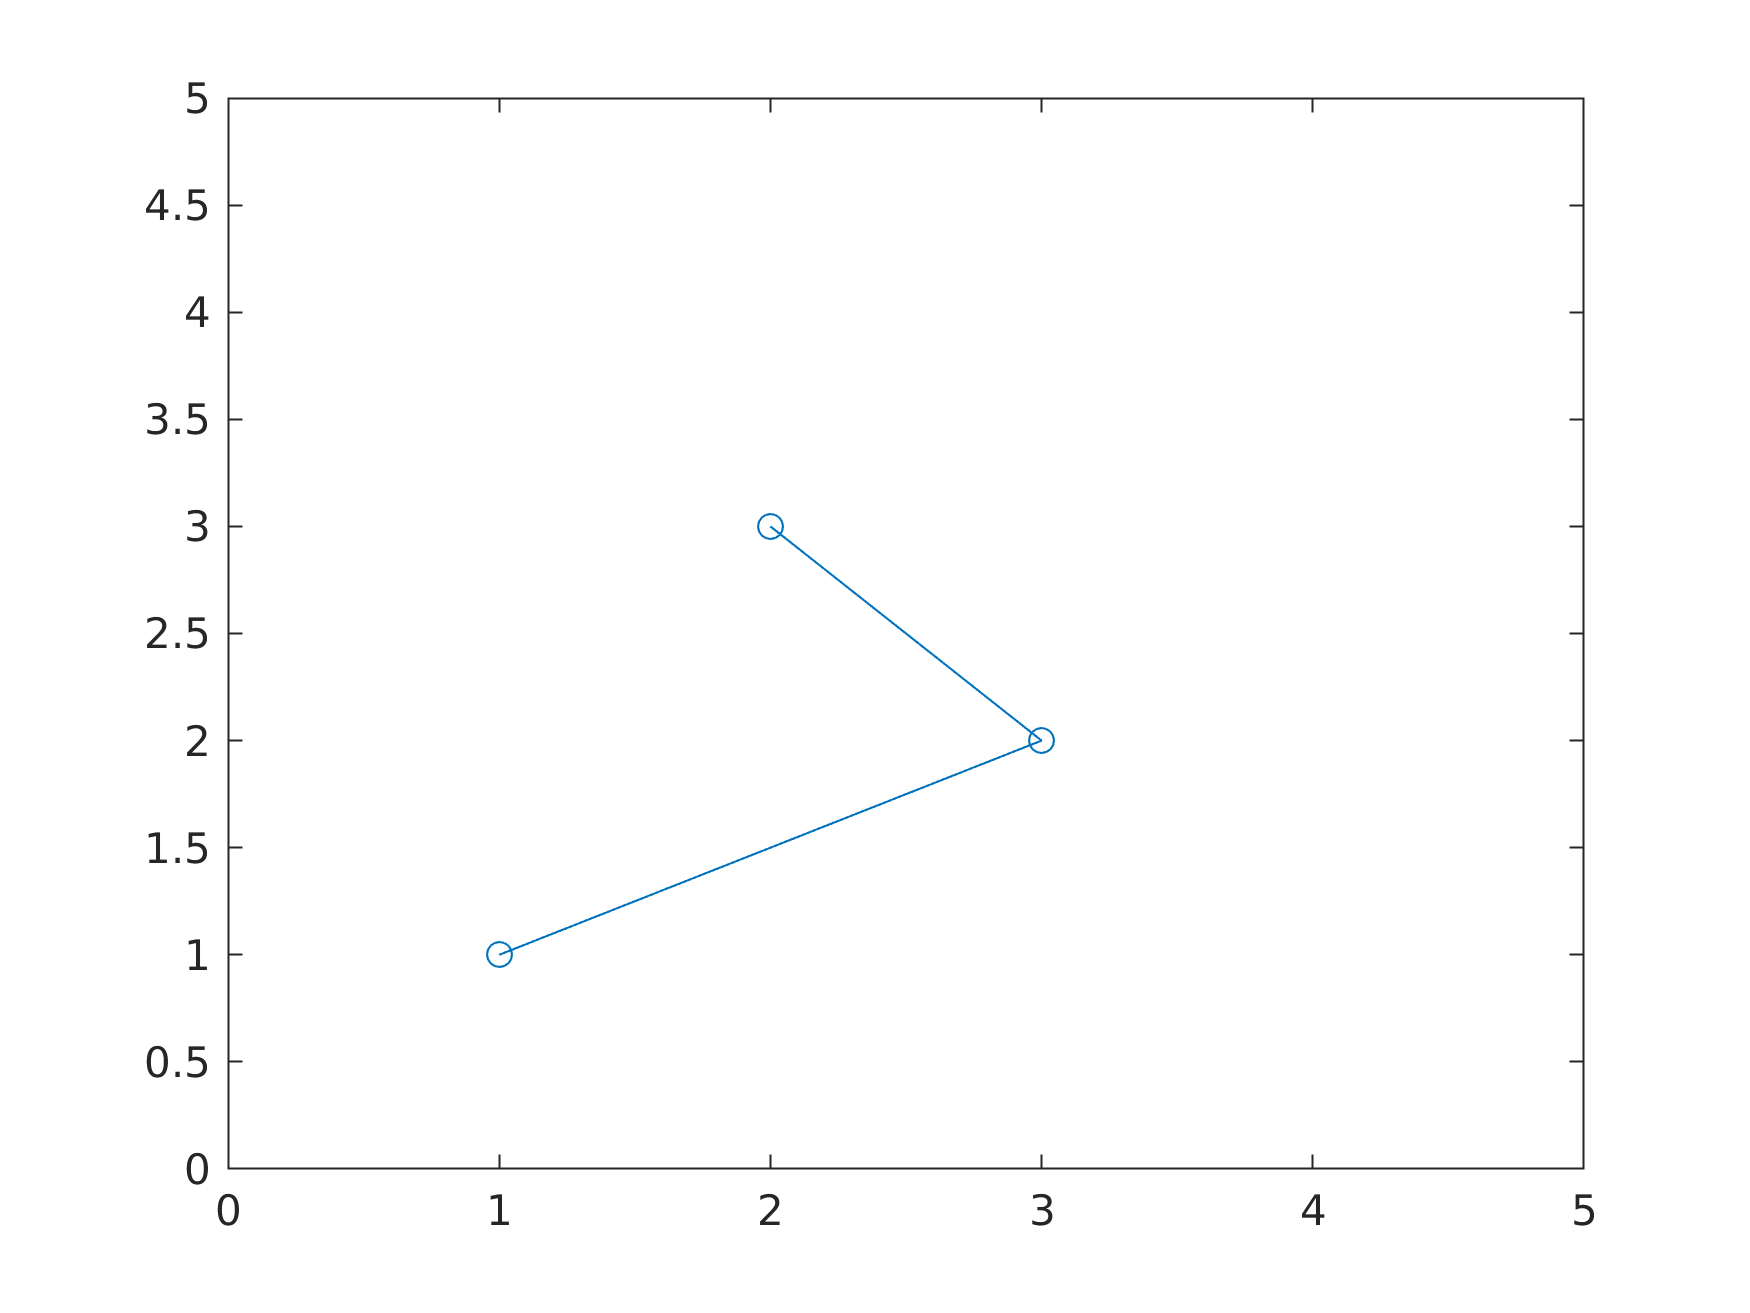
\includegraphics[width=8cm]{pic/basic_plotting_010.png}
\begin{hint}
The commands \verb!plot!, \verb!xlim! and \verb!ylim! can be useful.
\end{hint}
\begin{sol}
A solution is:
\begin{verbatim}
figure(1);
clf;
x = [1, 3, 2];
y = [1, 2, 3];
plot(x, y, '-o');
xlim([0, 5]);
ylim([0, 5]);
\end{verbatim}
\end{sol}
\end{ex}

\begin{ex}
Find a root of the function $f(x) = e^{-x} - x$.
\begin{hint}
The command \verb!fzero! can be useful.
\end{hint}
\begin{sol}
A solution is:
\begin{verbatim}
fh = @(x) exp(-x) - x
root1 = fzero(fh, 1)
\end{verbatim}
\end{sol}
\end{ex}

\begin{ex}
Find the minimum of the function $f(x) = e^x - 2x$.
\begin{hint}
The command \verb!fminsearch! can be useful.
\end{hint}
\begin{sol}
A solution is:
\begin{verbatim}
fh = @(x) -2x + exp(x);
fminsearch(fh, 1)
\end{verbatim}
\end{sol}
\end{ex}


\begin{ex}
Use the debugger to examine the \verb!binary_log! function.
\begin{enumerate}
\item Open the file \href{https://raw.githubusercontent.com/henrikmidtiby/matlab-notes/master/code/debugger_example_binary_log/binary_log.m}{binary.log}
\item	Insert a \verb!fprintf! statement in line 3, that prints the input arguments given to the function.
\item	Insert a breakpoint (red circle next to the line numbers) at the start of the function "\verb!binary_log!".
\item	Call the function as "\verb!binary_log(8)!" and step through the method using the debugger.
\item	Insert a comment in the function that explains what the while loop in line 6--9 is doing.
\item	Call the function as "\verb!binary_log(0.25)!" and step through the method using the debugger.
\item	Insert a comment in the function that explains what the while loop in line 11--14 is doing.
\end{enumerate}
\begin{hint}
Log rules to be aware of
\[
\log_2(2 \cdot a) = 1 + \log_2(a) \\
\log_2(a / 2) = -1 + \log_2(a)
\]
\end{hint}
\begin{sol}
Lines 6--9 applies the rule $\log_2(2 \cdot a) = 1 + \log_2(a)$ until $a$ is less than 2.

Lines 11--14 applies the rule $\log_2(a / 2) = -1 + \log_2(a)$ until $a$ is greater than or equal to 1.
\end{sol}
\end{ex}


\begin{ex}
Plot the functions $f(x) = e^x$ and $g(x) = 4x$ over the interval $x \in [-1, 3]$.
\begin{hint}
Define two function handles, one to each function.
Use the functions \verb!linspace!, \verb!hold on!, \verb!plot! and \verb!figure!.
\end{hint}
\begin{sol}
A solution is:
\begin{verbatim}
fh = @(x) exp(x);
gh = @(x) 4*x;
x = linspace(-1, 3);
figure(1);
clf;
hold on;
plot(x, fh(x));
plot(x, gh(x))
\end{verbatim}
\end{sol}
\end{ex}


\begin{ex}
Download the file \verb!test.csv! from this 
\href{https://raw.githubusercontent.com/henrikmidtiby/matlab-notes/master/code/loading_data/test.csv}{link}.
Load the data into matlab and plot the data.
\begin{hint}
\end{hint}
\begin{sol}
A solution is:
\begin{lstlisting}
\end{lstlisting}
\end{sol}
\end{ex}

\begin{ex}
Make the figure inserted below. Pay attention to the axes labels and the width of the plotted line. The visualized function is $f(x) = x^2 - x$. \par
\noindent
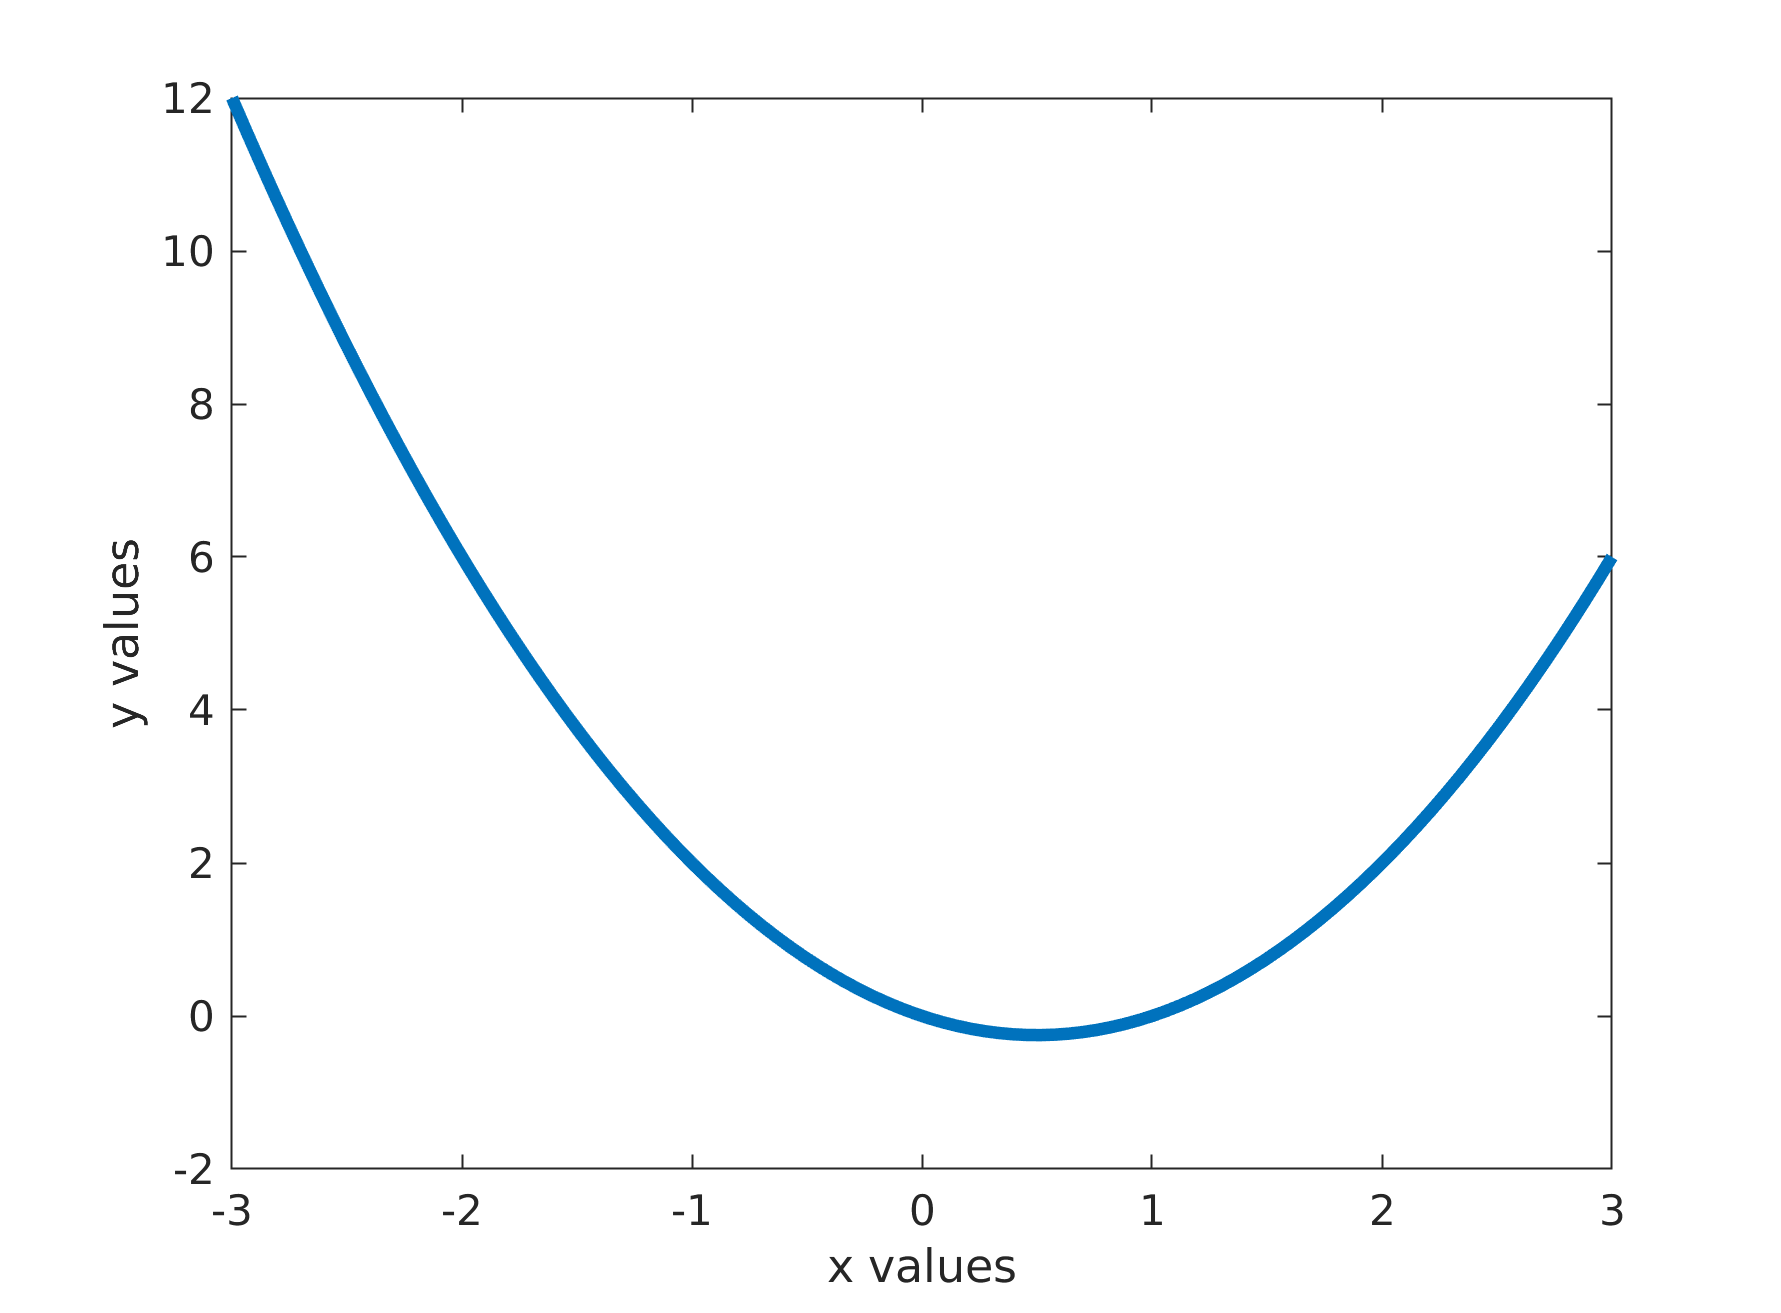
\includegraphics[width=8cm]{pic/basic_plotting_020.png}
\begin{hint}
The commands \verb!plot!, \verb!xlabel! and \verb!ylabel! can be useful.
\end{hint}
\begin{sol}
A solution is:
\begin{verbatim}
figure(1);
clf;
fh = @(x) -x + x.^2;
x = linspace(-3, 3);
plot(x, fh(x), 'LineWidth', 3);
xlabel('x values');
ylabel('y values');
\end{verbatim}
\end{sol}
\end{ex}


\begin{ex}
Find two numerical solutions to the equation
\[
e^{x} = 4x
\]
\begin{hint}
Write the equation on the form $f(x) = 0$ (collect all elements on the left hand side).
The command \verb!fzero! can be useful.
\end{hint}
\begin{sol}
A solution is:
\begin{verbatim}
fh = @(x) exp(x) - 4*x;
root1 = fzero(fh, 1)
root2 = fzero(fh, 3)
\end{verbatim}
\end{sol}
\end{ex}



\begin{ex}
Solve the set of linear equations
\begin{align*}
1	& = 5x + 2y	\\
0	& = -x + y + 3z + 2v	\\
-10 	& = x + 3y - 4z + v	\\
0	& = -2x + 3z - 2v 
\end{align*}
\begin{hint}
Write the system of equations on matrix form $A \cdot \vec{x} = \vec{b}$.
\end{hint}
\begin{sol}
A solution is:
\begin{verbatim}
A = [5, 2, 0, 0; -1, 1, 3, 2; 1, 3, -4, 1; -2, 0, 3, -2];
b = [1; 0; -10; 0];
x = linsolve(A, b)
A * x
\end{verbatim}
\end{sol}
\end{ex}



\begin{ex}
Enter\label{exPlotDataToFitLinearModelTo}
the following values for $x$ and $y$ and plot the points.
Then describe the trend you are observing in the data.
\begin{verbatim}
x = [1, 2, 3, 5];
y = [4, 3, 2, 1];
\end{verbatim}
\begin{hint}
Use the \verb!plot! method.
\end{hint}
\begin{sol}
A solution is:
\begin{verbatim}
x = [1, 2, 3, 5];
y = [4, 3, 2, 1];
figure(1);
clf;
plot(x, y, 'o');
\end{verbatim}
From the plot I see that the $y$ values decreases as the $x$ values increases.
\end{sol}
\end{ex}

\begin{ex}
This\label{exPlotDataToFitLinearModelTo2}
exercise is a continuation of exercise \ref{exPlotDataToFitLinearModelTo}.\\
Implement a linear model $y = a \cdot x + b$ in matlab. 
The linear model should be defined like below, where P is a vector containing the 
model parameters $a$ and $b$.
\begin{verbatim}
model = @(x, P) <fill in stuff here>;
\end{verbatim}
\begin{hint}
The output of the model should match the output below.
\begin{verbatim}
>> model([1, 2, 3, 5], [-1, 5])
ans =
     4     3     2     0
\end{verbatim}
\end{hint}
\begin{sol}
A solution is:
\begin{verbatim}
model = @(x, P) P(1) * x + P(2);
\end{verbatim}
\end{sol}
\end{ex}

\begin{ex}
This \label{exPlotDataToFitLinearModelTo3}
exercise is a continuation of exercise \ref{exPlotDataToFitLinearModelTo2}.\\
Implement a method that calculates the squared error
between the model and observations.
\[
\text{squared error} = \sum_i \left(y_i - \text{model}(x_i)\right)^2
\]
Assume that the $x$ and $y$ values are saved in the variables 
\verb!x! and \verb!y! respectively.
\begin{verbatim}
model_error = @(P) <fill in stuff here>;
\end{verbatim}
\begin{hint}
The \verb!sum! function is helpful.
\end{hint}
\begin{sol}
A solution is:
\begin{verbatim}
>> x = [1, 2, 3, 5];
>> y = [4, 3, 2, 1];
>> model = @(x, P) P(1) * x + P(2);
>> model_error = @(P) sum((y - model(x, P)).^2);
>> squared_error = model_error([-1.2, 5])
squared_error =
    4.5600
\end{verbatim}
\end{sol}
\end{ex}

\begin{ex}
This exercise is a continuation of exercise \ref{exPlotDataToFitLinearModelTo3}. \\
Minimize the squared error, defined in exercise \ref{exPlotDataToFitLinearModelTo3} 
and then plot the model with the 
found parameter values along with the original data.
\begin{hint}
You can try to minimize the function manually by calling it with different 
parameters and then adjust the parameters so that the function value
is reduced. It could look like this.
\begin{lstlisting}
>> squared_error = model_error([-1.2, 5])
squared_error = 4.5600
>> squared_error = model_error([-1.2, 4.5])
squared_error = 8.7600
>> squared_error = model_error([-1.2, 5.5])
squared_error = 2.3600
>> squared_error = model_error([-1.25, 5.5])
squared_error = 3.1875
>> squared_error = model_error([-1.15, 5.5])
squared_error = 1.7275
\end{lstlisting}


The \verb!fminsearch! function is helpful, it should converge to 
the proper solution independent of the initial guess.
The solution contains the following values $-0.7429$ and $4.5429$.
\end{hint}
\begin{sol}
A solution is:
\begin{verbatim}
x = [1, 2, 3, 5];
y = [4, 3, 2, 1];
model = @(x, P) P(1) * x + P(2);
model_error = @(P) sum((y - model(x, P)).^2);
P = fminsearch(model_error, [4, 2])

xvals = linspace(0, 6);
figure(1);
clf;
hold on;
plot(x, y, 'o');
plot(xvals, model(xvals, P));
\end{verbatim}
\end{sol}
\end{ex}



\begin{ex}
Plot the three functions given below in the same plot.
\[
f(x) = \frac{1}{x + 1} \qquad \qquad g(x) = \frac{1}{x + 3} \qquad \qquad h(x) = \frac{1}{(x + 1)(x + 3)}
\]
Do the functions have something in common?
\begin{hint}
Look at the discontinuities of the functions. Where are they placed?
\end{hint}
\begin{sol}
A solution is:
\begin{verbatim}
fh = @(x) 1 ./ (x + 1);
gh = @(x) 1 ./ (x + 3);
hh = @(x) 1 ./ ((x + 1) .* (x + 3));
x = linspace(-5, 1, 1000);
figure(1);
clf; 
hold on;
plot(x, fh(x));
plot(x, gh(x));
plot(x, hh(x));
ylim([-4, 4]);
\end{verbatim}
\end{sol}
\end{ex}

\begin{ex}
Given the three functions below:
\[
f(x) = \frac{1}{x + 1} \qquad \qquad g(x) = \frac{1}{x + 3} \qquad \qquad h(x) = \frac{1}{(x + 1)(x + 3)}
\]
Plot $h(x)$ and a linear combination of $f(x)$ and $g(x)$ in the same plot.
Adjust the coefficients of $f(x)$ and $g(x)$, so that the two plotted functions 
becomes as similar as possible.
\begin{hint}
An example of a linear combination of $f(x)$ and $g(x)$ is
\[
2 \cdot f(x) + 3 \cdot g(x)
\]
\end{hint}
\begin{sol}
A solution is:
\begin{verbatim}
fh = @(x) 1 ./ (x + 1);
gh = @(x) 1 ./ (x + 3);
hh = @(x) 1 ./ ((x + 1) .* (x + 3));
figure(2);
clf; 
hold on;
plot(x, 0.5*fh(x) - 0.5*gh(x));
plot(x, hh(x), 'LineStyle', '- -', 'LineWidth', 3);
ylim([-4, 4]);
\end{verbatim}
\end{sol}
\end{ex}




\section{Numerical integration}


\begin{ex}
Rewrite the following function such that it uses a for loop.

\begin{lstlisting}
function functionThatRepeatsStuff()
disp(1);
disp(1);
disp(1);
disp(1);
disp(1);
disp(1);
disp(1);
disp(1);
end
\end{lstlisting}
\begin{hint}
Identify what is repeated and how many times it is repeated.
\end{hint}
\begin{sol}
A solution is:
\begin{lstlisting}
function functionThatRepeatsStuff()
for k = 1:8
  disp(1);
end
end
\end{lstlisting}
\end{sol}
\end{ex}



\begin{ex}
Rewrite the following function such that it uses a for loop.
\begin{lstlisting}
function functionThatCounts()
disp(1);
disp(2);
disp(3);
disp(4);
disp(5);
disp(6);
disp(7);
disp(8);
disp(9);
end
\end{lstlisting}
\begin{hint}
Use a for loop, with a structure as shown here:
\begin{lstlisting}
for k = 1:4
end
\end{lstlisting}
\end{hint}
\begin{sol}
A solution is:
\begin{lstlisting}
function functionThatCounts()
for k = 1:9
  disp(k);
end
end
\end{lstlisting}
\end{sol}
\end{ex}



\begin{ex}
Create \label{exSumOfPositiveIntegersLessThanN}
a function that takes one positive integer, n, as argument and
calculates the sum of all integers in the range $1, 2, ..., n$.

\begin{lstlisting}
function res = sumOfIntegersLessThanOrEqualTo(n)
\end{lstlisting}
Example usage of the function:
\begin{lstlisting}
>> sumOfIntegersLessThanOrEqualTo(1);
>> sumOfIntegersLessThanOrEqualTo(1)
ans = 1
>> sumOfIntegersLessThanOrEqualTo(5)
ans = 15
>> sumOfIntegersLessThanOrEqualTo(10)
ans = 55
>> sumOfIntegersLessThanOrEqualTo(100)
ans = 5050
\end{lstlisting}
\begin{hint}
Use a for loop, with a structure as shown here:
\begin{lstlisting}
for k = 1:n
end
\end{lstlisting}
Prior to the for loop, create a variable and set its value to 0.
Then update the value in the variable for each cycle in the for loop.
\end{hint}
\begin{sol}
A solution is:
\begin{lstlisting}
function res = sumOfIntegersLessThanOrEqualTo(n)
res = 0;
for k = 1:n
  res = res + k;
end
end
\end{lstlisting}
\end{sol}
\end{ex}




\begin{ex}
Create a function that takes one positive integer, n, as argument and
calculates the sum of all integers in the range $1, 2, ..., n$, which are even.

\begin{lstlisting}
function res = sumOfEvenIntegersLessThanOrEqualTo(n)
\end{lstlisting}
Example usage of the function:
\begin{lstlisting}
>> sumOfEvenIntegersLessThanOrEqualTo(1);
>> sumOfEvenIntegersLessThanOrEqualTo(1)
ans = 0
>> sumOfEvenIntegersLessThanOrEqualTo(5)
ans = 6
>> sumOfEvenIntegersLessThanOrEqualTo(10)
ans = 30
>> sumOfEvenIntegersLessThanOrEqualTo(100)
ans = 2550
\end{lstlisting}
\begin{hint}
Modify the solution to exercise \ref{exSumOfPositiveIntegersLessThanN}
so it only increments the variable when $k$ is even.
\end{hint}
\begin{sol}
A solution is:
\begin{lstlisting}
function res = sumOfEvenIntegersLessThanOrEqualTo(n)
res = 0;
for k = 1:n
  if(mod(k, 2) == 0)
    res = res + k;
  end
end
end
\end{lstlisting}
\end{sol}
\end{ex}



\begin{ex}
Create a function that calculates the n'th Fibonacci number. The nth
fibonacci number can be calculated using the formula: 
\[
F_n = F_{n-1} + F_{n-2}
\]
with the two base cases $F_0 = 0$ and $F_1 = 1$. The sequence goes like
$0, 1, 1, 2, 3, 5, 8, 13, 21, 34, ...$
\begin{lstlisting}
function res = fib(n)
\end{lstlisting}
Example usage of the function:
\begin{lstlisting}
>> fib(0);
>> fib(0)
ans = 0
>> fib(1)
ans = 1
>> fib(6)
ans = 8
>> fib(17)
ans = 1597
>> fib(29)
ans = 514229
\end{lstlisting}
\begin{hint}
Use one or more if statements to ensure that the two base
cases are handled properly.
Then use the relation
\[
\textrm{fib}(n) = \textrm{fib}(n - 1) + \textrm{fib}(n - 2)
\]
\end{hint}
\begin{sol}
A solution is:
\begin{lstlisting}
function res = fib(n)

if(n < 2)
  res = n;
else
  res = fib(n - 1) + fib(n - 2);
end
end
\end{lstlisting}
\end{sol}
\end{ex}
\moved



\begin{ex}[Reference value]%
Evaluate the integral below numerically using the \verb!integral! function.
\[
\int_0^5 e^{-x} \cdot \sin(x) dx
\]
\begin{hint}
The two first significant digits are 0.50.
\end{hint}
\begin{sol}
A solution is:
\begin{verbatim}
fh = @(x) exp(-x) .* sin(x);
integral(fh, 0, 5)
\end{verbatim}
\end{sol}
\end{ex}

\begin{ex}[Trapez rule example]%
Create a list of 10 evenly spaced $x$--values from 
0 to 5, these values will be called $x_i$.
Evaluate \label{exTrapezRule}
the function 
\[
  e^{-x} \cdot \sin(x) dx
\]
at these $x$--values and save these values in 
a list called $y_i$.
Then calculate the sum
\[
\sum_{i = 1}^{9} \frac{y_i + y_{i + 1}}{2} \cdot (x_{i + 1} - x_i)
\]
\begin{hint}
Use \verb!linspace! to generate a list of x-values.
\end{hint}
\begin{sol}
\begin{lstlisting}
nvals = 10;
x = linspace(0, 5, nvals);

fh = @(x) exp(-x) .* sin(x);
fx = fh(x);

value = 0;
for k = 1:(nvals - 1)
    avg_height = 0.5*(fx(k) + fx(k + 1));
    dx = x(k + 1) - x(k);
    value = value + avg_height * dx;
end
\end{lstlisting}
\end{sol}
\end{ex}

\begin{ex}[Reduced step length]%
Repeat exercise \ref{exTrapezRule}, but use 20 steps instead of 10.
\begin{hint}
Look at the solution to \ref{exTrapezRule} and modify the call to linspace.
\end{hint}
\begin{sol}
\begin{lstlisting}
nvals = 20;
x = linspace(0, 5, nvals);

fh = @(x) exp(-x) .* sin(x);
fx = fh(x);

value = 0;
for k = 1:(nvals - 1)
    avg_height = 0.5*(fx(k) + fx(k + 1));
    dx = x(k + 1) - x(k);
    value = value + avg_height * dx;
end
\end{lstlisting}
\end{sol}
\end{ex}

\begin{ex}[Trapez rule as a function]%
Create a function that uses the Trapez rule to estimate the 
value of a definite integral (\href{https://en.wikipedia.org/wiki/Trapezoidal_rule}{wikipedia article}).
The function must have the signature
\begin{lstlisting}
function res = trapez_rule(fh, x_low, x_high, n_intervals)
\end{lstlisting}
where \verb!fh! is a function handle, 
\verb!x_low! and \verb!x_high! are the integration limits
and \verb!n_intervals! is the number of subintervals 
used for evaluating the integral.
Use the following examples to test the function
\begin{lstlisting}
>> trapez_rule(fh, 0, 5, 10)
ans = 0.4770
>> trapez_rule(fh, 0, 5, 20)
ans = 0.4966
>> trapez_rule(fh, 0, 5, 100)
ans = 0.5021
\end{lstlisting}
\begin{hint}
Use your solution from exercise \ref{exTrapezRule} and build a function around it.
\end{hint}
\begin{sol}
A solution is:
\begin{lstlisting}
function res = trapez_rule(fh, x_low, x_high, n_intervals)

x = linspace(x_low, x_high, n_intervals);
fx = fh(x);
res = 0;
for k = 1:(n_intervals - 1)
    avg_height = 0.5*(fx(k) + fx(k + 1));
    dx = x(k + 1) - x(k);
    res = res + avg_height * dx;
end

end
\end{lstlisting}
\end{sol}
\end{ex}
\moved


\begin{ex}
Estimate the values of the integrals
\[
V_1 = \int_1^3 \sin(2x) \, dx \qquad \textrm{and} \qquad
V_2 = \int_2^6 \frac{\sin(x)}{2} \, dx.
\]
How would you expect them to be related?
\begin{hint}
Use the \verb!integral! function.
The substitution rule has been applied to the first
integral and this has generated the second integral.
\end{hint}
\begin{sol}
\begin{lstlisting}
fh1 = @(x) sin(2*x);
fh2 = @(x) sin(x) / 2;
integral(fh1, 1, 3)
integral(fh2, 2, 6)
\end{lstlisting}
\end{sol}
\end{ex}



\section{Numerical solutions of differential equations}


\subsection{Euler's method}


\begin{ex}[Eulers method]%
Function definition:
\begin{lstlisting}
function [yvals, fcalls] = euler(fnc, xvals, y0)
% Uses the Euler method for approximating the first order
% differential equation defined by the function handle fnc.
%
% Input values:
% - fnc Function handle to a function which takes two
% input arguments and returns a scalar value.
% Eg. @(x, y) (y+sin(x))
% - xvals List of x values where the corresponding y
% values should be calculated.
% - y0 Initial state of the dependent function.
%
% Output values:
% - yvals Approximation of y(x) at the locations
% specified in xvals.
% - fcalls Number of function evaluations.
\end{lstlisting}
Example usage of the function:
\begin{lstlisting}
>> [yvals, fevals] = euler(@(x, y) y, [0:5], 1)
yvals =
1 2 4 8 16 32
fevals =
5
>> euler(@(x, y) y, [0:5], 2)
ans =
2 4 8 16 32 64
>> euler(@(x, y) 0.1*y, [0:5], 1)
ans =
1.0000 1.1000 1.2100 1.3310 1.4641 1.6105
>> euler(@(x, y) 0.1*y+0.2*x, [0:5], 1)
ans =
1.0000 1.1000 1.4100 1.9510 2.7461 3.8207
\end{lstlisting}
\begin{hint}
No hint provided yet.
\end{hint}
\begin{sol}
No solution provided yet.
\end{sol}
\end{ex}

\begin{ex}
\label{excEulerConvergence} \\
For the initial value problem
\begin{align}
y'(t)
	& = 1.2 \cdot y(t) 	&
y(0) = 1
\end{align}
Determine the analytic solution and calculate the exact value of $y(3)$.
Use Euler's method to approximate $y(3)$ with different step lengths $h$.
How is the error related to the used step length?
\begin{hint}
No hint provided yet.
\end{hint}
\begin{sol}
No solution provided yet.
\end{sol}
\end{ex}



\todo[inline]{Add exercises about secret sharing. Get inspiration from this video: Secret Sharing Explained Visually \url{https://www.youtube.com/watch?v=iFY5SyY3IMQ}}


\section{More functions}

\begin{ex}
A store want to implement a 10\% discount to customers 
buying for 600 kr or more.
Create a function that implements the discount calculation
described above, the function must have the signature:
\begin{lstlisting}
function actual_price = apply_discount(ordinary_price)
\end{lstlisting}
Use the following examples to test the function.
\begin{lstlisting}
>> apply_discount(100)
ans = 100
>> apply_discount(600)
ans = 540
>> apply_discount(1000)
ans = 900
>> apply_discount(134)
ans = 134
\end{lstlisting}
\begin{hint}
Use an \verb!if! statement to choose whether the 
discount should be applied or not.
\end{hint}
\begin{sol}
A solution is:
\begin{lstlisting}
function actual_price = apply_discount(ordinary_price)

if(ordinary_price >= 600)
    actual_price = 0.9*ordinary_price;
else
    actual_price = ordinary_price;
end

end
\end{lstlisting}
\end{sol}
\end{ex}




\begin{ex}
\label{exCalcMean}%
Create a function that calculates the mean value $\overline{x}$ of a list of numbers.
\begin{align}
\overline{x}
	& = \frac{1}{N} \sum_{i = 1}^{N} x_i
\end{align}
The function signature should be:
\begin{lstlisting}
function mean_value = calcMean(list)
\end{lstlisting}
Use the following examples to test the function:
\begin{lstlisting}
>> calcMean([1]);
>> calcMean([1])
ans = 1
>> calcMean([1, 3])
ans = 2
>> calcMean([-1, 7])
ans = 3
\end{lstlisting}
\begin{hint}
Use a for loop to sum all values.
\end{hint}
\begin{sol}
A solution is:
\begin{lstlisting}
function mean_value = calcMean(list)

% Initialize counters
total = 0;
n_elements = 0;

% Iterate over values in the list
for value = list
    total = total + value;
    n_elements = n_elements + 1;
end

% Calculate the mean value
mean_value = total / n_elements;

end
\end{lstlisting}
\end{sol}
\end{ex}




\begin{ex}
\label{exMinOfThree}%
Create a function which takes three input arguments
(assumed to be numerical values) and returns the 
minimum value of the three input values.
The function must have the signature:
\begin{lstlisting}
function minval = min_of_three(a, b, c)
\end{lstlisting}
Use the following examples to test the function.
\begin{lstlisting}
>> min_of_three(1, 2, 3)
ans = 1
>> min_of_three(100, 2, 3)
ans = 2
>> min_of_three(-1, 2, -3)
ans = -3
\end{lstlisting}
\begin{hint}
Use two \verb!if! statements to locate the minimal element.
\end{hint}
\begin{sol}
A solution is:
\begin{lstlisting}
function minval = min_of_three(a, b, c)

minval = a;

if(b < minval)
    minval = b;
end

if(c < minval)
    minval = c;
end

end
\end{lstlisting}
\end{sol}
\end{ex}

\begin{ex}
\label{exThreeForThePriceOfTwo}%
A store want to offer a buy three items and pay for two items 
discount (the customer should pay for the two most 
expensive items).
Create a function that takes three input values (the price of the individual items) and returns the total price after taking 
the discount into account.
The function signature should be:
\begin{lstlisting}
function total_price = buy_three_pay_for_two(a, b, c)
\end{lstlisting}
Use the following examples to test the function:
\begin{lstlisting}
>> buy_three_pay_for_two(10, 20, 10)
ans = 30
>> buy_three_pay_for_two(10, 20, 30)
ans = 50
>> buy_three_pay_for_two(30, 20, 35)
ans = 65
\end{lstlisting}
\begin{hint}
The function \verb!min_of_tree! from exercise \ref{exMinOfThree} 
can simplify the calculation.
\end{hint}
\begin{sol}
A solution is:
\begin{lstlisting}
function total_price = buy_three_pay_for_two(a, b, c)

total_price = a + b + c - min_of_three(a, b, c);

end
\end{lstlisting}
\end{sol}
\end{ex}



\begin{ex}
\label{exCalcSquaredMean}%
Create a function that calculates the mean squared value $\overline{x^2}$ of a list of
numbers.
\begin{align}
\overline{x^2}
	& = \frac{1}{N} \sum_{i = 1}^{N} x_i^2
\end{align}
The function signature should be:
\begin{lstlisting}
function res = calcSquaredMean(list)
\end{lstlisting}
Use the following examples to test the function:
\begin{lstlisting}
>> calcSquaredMean([1]);
>> calcSquaredMean([1])
ans = 1
>> calcSquaredMean([1, 3])
ans = 5
>> calcSquaredMean([-1, 7])
ans = 25
\end{lstlisting}
\begin{hint}
Use a for loop to sum the square of all values.
\end{hint}
\begin{sol}
A solution is:
\begin{lstlisting}
function mean_value = calcSquaredMean(list)

% Initialize counters
total = 0;
n_elements = 0;

% Iterate over values in the list
for value = list
    total = total + value^2;
    n_elements = n_elements + 1;
end

% Calculate the mean value
mean_value = total / n_elements;

end
\end{lstlisting}
\end{sol}
\end{ex}




\begin{ex}
Create a function, that takes a list a input and returns every third element from that list.
The function signature should be:
\begin{lstlisting}
function res = return_every_third_element(list)
\end{lstlisting}
Use the following examples to test the function:
\begin{lstlisting}
>> return_every_third_element([1, 2, 3, 4])
ans = 3
>> return_every_third_element([1])
ans = []
>> return_every_third_element([1, 2, 3, 4, 3, 2])
ans = 3     2
\end{lstlisting}
\begin{hint}
The modulus function \verb!mod! can be of great help
when combined with a \verb!for! loop and an \verb!if! statement.

To add (append) a new element to an existing list, 
use the following code
\begin{lstlisting}
res = []; % Create an empty list.
res = [res, 3]; % Append the value 3 to the list.
\end{lstlisting}
\end{hint}
\begin{sol}
A solution is:
\begin{lstlisting}
function res = return_every_third_element(list)

res = [];
for k = 1:length(list)
    if(mod(k, 3) == 0)
        res = [res, list(k)];
    end
end

end
\end{lstlisting}
\end{sol}
\end{ex}


\begin{ex}
The store from exercise \ref{exThreeForThePriceOfTwo}, would like
to extend the three for the price of two offer, to all items
in the customers shopping basket.
Create a new function that calculates the total price through 
the following steps:
\begin{enumerate}
\item	sort the list of item prices in decreasing order
\item	extract every third element from the list
\item	calculate the sum of all items in the original list (total sum)
\item	calculate the total discount by adding every third element from the sorted list
\item 	calculate the final price by subtracting the sum of thirds from the total sum
\end{enumerate}
The function signature should be:
\begin{lstlisting}
function final_price = three_for_two_offer_many_items(list)
\end{lstlisting}
Use the following examples to test the function:
\begin{lstlisting}
>> three_for_two_offer_many_items([1, 2, 3])
ans = 5
>> three_for_two_offer_many_items([1, 2, 3, 1, 2, 3])
ans = 9
>> three_for_two_offer_many_items([1, 2, 3, 1, 2, 3, 1, 2, 3])
ans = 12
\end{lstlisting}
\begin{hint}
Use the option ``descend'' to the \verb!sort! function.
\end{hint}
\begin{sol}
A solution is:
\begin{lstlisting}
\end{lstlisting}
\end{sol}
\end{ex}


\subsection{Function handles}

We have earlier worked with functions that take numbers and lists 
as input arguments.
But a function can also take a function handle as input argument.
A function handle is a reference to a specific function. 
In the example below is a reference to the sinus function created 
and later tested.
%
\begin{lstlisting}
>> functionHandle = @sin;
>> functionHandle(0.123)
ans = 0.1227
>> sin(0.123)
ans = 0.1227
\end{lstlisting}
%
A function handle can also be generated without using an existing function as template.
The following syntax lets you create function handles from scratch.
%
\begin{lstlisting}
@(input parameters) code to calculate result
\end{lstlisting}
%
As an example the second order taylor expansion for $\cos(x)$ is used to create 
a function handle.
\begin{lstlisting}
>> fh = @(x) 1 - 0.5*x.^2;
>> cos([0, 0.1, 0.3])
ans = 1.0000    0.9950    0.9553
>> fh([0, 0.1, 0.3])
ans = 1.0000    0.9950    0.9550
\end{lstlisting}

\begin{ex}
Create a function handle named \emph{sumOfSineAndCosine} for the expression
\begin{align*}
f(x) & = \sin(x) + \cos(x)
\end{align*}
Example usage of the function:
\begin{lstlisting}
>> sumOfSineAndCosine([0, 0.1, 0.2, 0.3, 1])
ans = 1.0000    1.0948    1.1787    1.2509    1.3818
\end{lstlisting}
\begin{hint}
Use the syntax
\begin{lstlisting}
fname = @(x) expression;
\end{lstlisting}
Where \verb!fname! and \verb!expression! should be modified.
\end{hint}
\begin{sol}
To create the function handle, run the code below in the matlab command window.
\begin{lstlisting}
sumOfSineAndCosine = @(x) sin(x) + cos(x);
\end{lstlisting}
\end{sol}
\end{ex}



\begin{ex}
Create a function that takes a function handle and a list as input arguments.
The output should be a list with the same number of elements as the input list.
The values in the output list should be the value returned by the function handle 
when applied to the corresponding element in the input list.
The function signature should be:
\begin{lstlisting}
function res = applyFunctionHandleToList(fh, list)
\end{lstlisting}
Example usage of the function:
\begin{lstlisting}
>> applyFunctionHandleToList(@(x) 1, [1, 3, 9])
ans = 1     1     1
>> applyFunctionHandleToList(@(x) 1-x, [1, 3, 9])
ans = 0    -2    -8
\end{lstlisting}
\begin{hint}
Use a for loop to iterate over the input list.
\end{hint}
\begin{sol}
A solution is:
\begin{lstlisting}
function res = applyFunctionHandleToList(fh, list)

res = list;
for idx = 1:length(list)
	res(idx) = fh(list(idx));
end

end
\end{lstlisting}
\end{sol}
\end{ex}












\newpage
\section{Functions with if, for and while structures}

\begin{ex}
Create a function which takes a list and a pivot element 
as input. 
Elements in the list that are smaller than the pivot element
should be put in \verb!list1! and elements larger than or equal
should be put in \verb!list2!.
The function signature should be:
\begin{lstlisting}
function [list1, list2] = divide_by_pivot(list, pivot)
\end{lstlisting}
Use the following examples to test the function:
\begin{lstlisting}
>> [l1, l2] = divide_by_pivot([2, 6, 4], 3)
l1 = 2
l2 = 6     4
>> [l1, l2] = divide_by_pivot([2, 6, 4, 1, 4], 7)
l1 = 2     6     4     1     4
l2 = []
>> [l1, l2] = divide_by_pivot([2, 6, 4, 1, 4], 3)
l1 = 2     1
l2 = 6     4     4
\end{lstlisting}
\begin{hint}
Use a for loop to iterate over all elements in the input 
list.
Use an if statement to select which list the element should 
be added to.
\end{hint}
\begin{sol}
A solution is:
\begin{lstlisting}
function [list1, list2] = divide_by_pivot(list, pivot)

list1 = [];
list2 = [];
for val = list
    if val < pivot
        list1 = [list1, val];
    else
        list2 = [list2, val];
    end
end

end
\end{lstlisting}
\end{sol}
\end{ex}

\begin{ex}
Create a function that takes a list as input.
All elements in the list larger than zero should 
be put in a list that is then returned.

The function signature should be:
\begin{lstlisting}
function list = keep_positive_elements(input_list)
\end{lstlisting}
Use the following examples to test the function:
\begin{lstlisting}
>> keep_positive_elements([1, -2, 3, -4, 5])
ans = 1     3     5
>> keep_positive_elements([-1, -2, -3, -4, 5])
ans = 5
>> keep_positive_elements([6, 4, 2, 1])
ans = 6     4     2     1
\end{lstlisting}
\begin{hint}
Use a for loop to iterate over all values in 
the input list.
Use an if statement to decide whether the value
should be added to the output.
\end{hint}
\begin{sol}
A solution is:
\begin{lstlisting}
function list = keep_positive_elements(input_list)

list = [];
for val = input_list
    if val > 0
        list = [list, val];
    end
end

end
\end{lstlisting}
\end{sol}
\end{ex}


\begin{ex}
Create a function that takes a list of $n$ points as input 
(in the form of a $n$ by $2$ matrix).
The function should return a matrix with distances between 
the input points, so the element $a_{12}$ in the matrix 
contains the distance between the first and the second point
in the input list.
The function signature should be:
\begin{lstlisting}
function res = distance_matrix(list_of_points)
\end{lstlisting}
Use the following examples to test the function:
\begin{lstlisting}
>> distance_matrix([1, 0; 1, 1])
ans =
     0     1
     1     0
>> distance_matrix([1, 0; 0, 1; 1, 1])
ans =
         0    1.4142    1.0000
    1.4142         0    1.0000
    1.0000    1.0000         0
>> distance_matrix([1, 0; 1, 1; 4, 4])
ans =
         0    1.0000    5.0000
    1.0000         0    4.2426
    5.0000    4.2426         0
\end{lstlisting}
\begin{hint}
To calculate the distance matrix, all combinations
of two points should be examined.
This can be achieved by using two for loops placed 
inside each other (so you have an outer loop and an 
inner loop).
\end{hint}
\begin{sol}
A solution is:
\begin{lstlisting}
function res = distance_matrix(list_of_points)

[s1, s2] = size(list_of_points);
res = zeros(s1, s1);

for idx1 = 1:s1
    for idx2 = 1:s1
        p1 = list_of_points(idx1, :);
        p2 = list_of_points(idx2, :);
        difference = p1 - p2;
        distance = norm(difference);
        res(idx1, idx2) = distance;
    end
end

end
\end{lstlisting}
\end{sol}
\end{ex}


\begin{ex}
Create a function which takes two lists as input.
The output should be the two lists combined, 
so that all elements in the first list appears
before all elements in the second list.

The function signature should be:
\begin{lstlisting}
function res = concatenate_lists(list1, list2)
\end{lstlisting}
Use the following examples to test the function:
\begin{lstlisting}
>> concatenate_lists([1, 2, 3], [4, 5])
ans =
     1     2     3     4     5
>> concatenate_lists([5, 4], [1, 2, 3])
ans =
     5     4     1     2     3
\end{lstlisting}
\begin{hint}
Use a while loop to move all elements from list1 
to the output list.
Then use a new while loop to move all elements from 
list2 to the output list.
\end{hint}
\begin{sol}
A solution is:
\begin{lstlisting}
function res = concatenate_lists(list1, list2)

res = [];
idx = 1;
while idx <= length(list1)
    res = [res, list1(idx)];
    idx = idx + 1;
end

idx = 1;
while idx <= length(list2)
    res = [res, list2(idx)];
    idx = idx + 1;
end

end
\end{lstlisting}
\end{sol}
\end{ex}


\begin{ex}
\label{exSecantMethodOneStep}%
Implement a function that takes a function handle, and two 
$x$ values.
Use one step of the secant method to make an improved guess of the
root of a function, by using the two $x$ values as guesses.
The calculation to be done in the function is the following
where $f(x)$ is the function specified by the function handle
applied to the value $x$, and $x_1$ and $x_2$ are the two
guesses.
\[
x=x_{2}-f(x_{2}){\frac {x_{2}-x_{1}}{f(x_{2})-f(x_{1})}}.
\]
You can read more about the secant method on \href{https://en.wikipedia.org/wiki/Secant_method}{wikipedia}.

The function signature should be:
\begin{lstlisting}
function [x_improved, fval] = sekant_one_step(fh, x1, x2)
\end{lstlisting}
Use the following examples to test the function:
\begin{lstlisting}
>> [x, v] = sekant_one_step(@cos, 1, 2)
x = 1.5649
v = 0.0059
>> [x, v] = sekant_one_step(@cos, 2, 1.5649)
x = 1.5710
v = -1.8238e-04
>> [x, v] = sekant_one_step(@tan, 3, 3.5)
x = 3.1378
v = -0.0038
>> [x, v] = sekant_one_step(@tan, 3.5, 3.1478)
x = 3.1419
v = 2.7253e-04
\end{lstlisting}
\begin{hint}
No if, for or while loop is needed in this exercise.
\end{hint}
\begin{sol}
A solution is:
\begin{lstlisting}
function [x_improved, fval] = sekant_one_step(fh, x1, x2)

fx1 = fh(x1);
fx2 = fh(x2);

slope = (fx2 - fx1) / (x2 - x1);

x_improved = x2 - fx2 / slope;
fval = fh(x_improved);

end
\end{lstlisting}
\end{sol}
\end{ex}


\begin{ex}
Implement a function which takes a function handle, two $x$ 
values and a limit value as input.
Use the function implemented in exercise
\ref{exSecantMethodOneStep} to improve the root estimates.
Apply the function until the absolute value of the function 
evaluated at the best guess gets below the limit value.
Then return the improved guess, the value of the function 
evaluated at that guess and the number of
iterations used.

The function signature should be:
\begin{lstlisting}
function [x1, fvalue, iterations] = ...
    sekant_method(fh, x0, x1, limit)
\end{lstlisting}
Use the following examples to test the function:
\begin{lstlisting}
>> [x, fval, niter] = sekant_method(...
    @cos, 1.2, 2, 0.01)
x = 1.5724
fval = -0.0016
niter = 1
>> [x, fval, niter] = sekant_method(...
    @sin, 3, 4, 0.01)
x = 3.1395
fval = 0.0021
niter = 2
>> [x, fval, niter] = sekant_method(...
    @sin, 3, 4, 0.001)
x = 3.1416
fval = -7.4395e-08
niter = 3
>> [x, fval, niter] = sekant_method(...
    @(x) log(x) - 1, 3, 4, 0.001)
x = 2.7184
fval = 5.6055e-05
niter = 3
\end{lstlisting}
\begin{hint}
Use a while loop to repeat the calculations as many times 
as needed until the function value gets below the 
specified limit value.
\end{hint}
\begin{sol}
A solution is:
\begin{lstlisting}
function [x1, fvalue, iterations] = sekant_method(fh, x0, x1, limit)

iterations = 0;
fvalue = fh(x1);
while abs(fvalue) > limit
    [x2, fvalue] = sekant_one_step(fh, x0, x1);
    x0 = x1;
    x1 = x2;
    iterations = iterations + 1;
end

end
\end{lstlisting}
\end{sol}
\end{ex}


\begin{ex}
Implement a function that takes two lists
with numerical values as input.
Both lists are sorted, so their values are in 
increasing order.
The two lists should be merged together
in a single list such that the values in 
that list is also sorted.

The function signature should be:
\begin{lstlisting}
function res = merge_ordered_lists(list1, list2)
\end{lstlisting}
Use the following examples to test the function:
\begin{lstlisting}
>> merge_ordered_lists([1, 2, 4], [3, 7, 8])
ans = 1     2     3     4     7     8
>> merge_ordered_lists([1, 2, 4], [])
ans = 1     2     4
>> merge_ordered_lists([], [1, 2, 4])
ans = 1     2     4
\end{lstlisting}
\begin{hint}
Use three while loops.
The first while loop extracts the lowest value from 
the two lists and inserts it in the result.
The loops ends when all values have been used from 
one of the lists.
The second while loop moves all the remaining elements 
in list one to the result.
The third while loop moves all the remaining elements 
in list two to the result.
\end{hint}
\begin{sol}
A solution is:
\begin{lstlisting}
function res = merge_ordered_lists(list1, list2)

res = [];
idx1 = 1;
idx2 = 1;

while idx1 <= length(list1) && idx2 <= length(list2)
    if list1(idx1) < list2(idx2)
        res = [res, list1(idx1)];
        idx1 = idx1 + 1;
    else
        res = [res, list2(idx2)];
        idx2 = idx2 + 1;
    end
end

while idx1 <= length(list1)
    res = [res, list1(idx1)];
    idx1 = idx1 + 1;
end

while idx2 <= length(list2)
    res = [res, list2(idx2)];
    idx2 = idx2 + 1;
end

end
\end{lstlisting}
\end{sol}
\end{ex}



\begin{ex}
Create a function that takes a list of points and a query point
as input.
The function should then determine the point from the 
input list that is nearest the query point.
The index of the nearest point and the distance to the 
query point should then be returned.

The function signature should be:
\begin{lstlisting}
function [min_dist_idx, min_distance] = ...
    locate_nearest_point(input_list, query_point)
\end{lstlisting}
Use the following examples to test the function:
\begin{lstlisting}
>> [idx, dist] = locate_nearest_point([1, 1; 1, 5], [1.1, 1])
idx = 1
dist = 0.1000
>> [idx, dist] = locate_nearest_point([1, 1; 1, 5; 5, 4], [2, 4])
idx = 2
dist = 1.4142
>> [idx, dist] = locate_nearest_point([1, 1; 1, 5], [2, 4])
idx = 2
dist = 1.4142
\end{lstlisting}
\begin{hint}
Use a for loop to iterate over all points in the list of points.
For each point in the list, calculate the distance to the 
reference point and save the index of the point and the
distance to it, if it is the smallest distance seen thus far.
\end{hint}
\begin{sol}
A solution is:
\begin{lstlisting}
function [min_dist_idx, min_distance] = ...
    locate_nearest_point(input_list, query_point)

min_dist_idx = -1;
min_distance = 100000000;

for idx = 1:size(input_list, 1)
    point = input_list(idx, :);
    difference = point - query_point;
    distance = norm(difference);
    if distance < min_distance
        min_dist_idx = idx;
        min_distance = distance;
    end
end

end
\end{lstlisting}
\end{sol}
\end{ex}


\newpage
\section{2019-11-25 Numerical root finding}

\todo[inline]{Add exercises about plotting phase space diagrams for differential equations}
\todo[inline]{Examine the stability about equilibria in differential equations}

In the next set of exercises the goal will be to find solutions to the equation
%
\begin{align}
x
	& = \exp(x - 2)
\end{align}
%
The first step is to rewrite the equation such that one of the sides become 0.
%
\begin{align}
0
	& = \exp(x - 2) - x
\end{align}
%
The right hand side will be denoted $f(x)$ and the problem is now to find the 
roots of the function $f(x)$.
\begin{align}
0 & = f(x)
\end{align}

\begin{ex}
Locate the two roots of the function graphically using the plot command in matlab.
To ensure precise readings use the zoom functionality.
Give the roots with at least three correct decimals.
\end{ex}


\subsection{Fixed point iteration}

\begin{align}
f_0(x_0)
	& = f(x_0)	\\
f_n(x_0)
	& = f_{n - 1}(x_0)
\end{align}


\begin{ex}
Create a function which performs fixed point iterations on a given
function.
The function should take three input arguments, a function handle $f$, the initial x value 
($x_0$) and the number of iterations ($n$).
The return value should be $f_n(x_0)$.
The intermediate calculations $f_0(x_0)$, $f_1(x_0)$, $f_2(x_0)$, \ldots 
should be displayed on screen.

\begin{lstlisting}
function res = fixedIter(x0, n)
\end{lstlisting}
Example usage of the function:
\begin{lstlisting}
>> fnc = @(x) exp(x - 2);
>> fixedIter(fnc, 1, 2)
    0.3679
    0.1955
    0.1646
ans =
    0.1646
\end{lstlisting}
\end{ex}

\begin{ex}
Does the function fixedIter always converge to the same value when used on the function
handle given in the exercise above?
If the function converges, how is the converged value related 
to the equation $x = \exp(x - 2)$?
\end{ex}




\begin{ex}
Implement a function which uses bisection to locate roots in a given function. 
As input should it take a function handle, the initial interval (given as 
lower and higher values) and the number of iterations.
If the function have opposite signs at the lower and higher values the 
bisection method should run, in the other case a warning should be issued.
As output the function should return an array containing four columns and a number of 
rows equal to the number of iterations.
Each row should have the values \emph{lower}, \emph{higher}, \emph{fvalLower} and 
\emph{fvalHigher} (the current limits and the function values at the limits).
 
\begin{lstlisting}
function data = bisection(fnc, lower, higher, iterations)
\end{lstlisting}
Example usage of the function:
\begin{lstlisting}
>> fnc = @(x) exp(x - 2) - x;
>> bisection(fnc, 0, 0.1, 5)
Bad starting values
ans =[]
>> bisection(fnc, 0, 1, 5)
ans =
         0    0.5000    0.1353   -0.2769
         0    0.2500    0.1353   -0.0762
    0.1250    0.2500    0.0284   -0.0762
    0.1250    0.1875    0.0284   -0.0243
    0.1563    0.1875    0.0020   -0.0243
\end{lstlisting}
\end{ex}


\begin{ex}\\
Investigate how the bisection method converges. 
E. g. how many iterations is required to reach a given accuracy?
\end{ex}

\begin{ex}
Implement a function which uses the secant method to locate roots in a given function.
As input should it take a function handle and two different $x$ values near the root 
that should be located and the number of iterations.
If the method converges before the requested number of iterations it should halt 
(the method has converged when the calculated function value is zero).
After each iteration the method should output the new estimate of the root location $x$
and the function value at $x$.
The secant method is described here \url{http://en.wikipedia.org/wiki/Secant_method}.

\begin{lstlisting}
function secant(fnc, x0, x1, iterations)
\end{lstlisting}
Example usage of the function:
\begin{lstlisting}
>> fnc = @(x) exp(x - 2) - x;
>> format long
>> secant(fnc, 3, 3.4, 3)
   3.400000000000000   0.655199966844675
   3.120274401785570  -0.054579081629965
   3.141784146672724  -0.009432188618255
>> secant(fnc, 0.1, 0.2, 9)
   0.200000000000000  -0.034701111778413
   0.158821380623629  -0.000191029545640
   0.158593437586678   0.000000758928080
   0.158594339582341  -0.000000000016240
   0.158594339563039                   0
\end{lstlisting}
\end{ex}



\begin{ex}\\
Implement a function which uses the regula falsi method locate roots in a given function.
As input should it take a function handle, the initial interval (given as 
lower and higher values) and the number of iterations.
If the function has opposite signs at the lower and higher values the 
regula falsi method should run, in the other case a warning should be issued.
As output the function should return an array containing four columns and a number of 
rows equal to the number of iterations.
Each row should have the values \emph{lower}, \emph{higher}, \emph{fvalLower} and 
\emph{fvalHigher} (the current limits and the function values at the limits).

\begin{lstlisting}
function regulafalsi(fnc, lower, higher, iterations)
\end{lstlisting}
Example usage of the function:
\begin{lstlisting}
>> fnc = @(x) exp(x - 2) - x;
>> regulafalsi (fnc, 0 ,  -1,  5)
Bad starting values
ans = []
>> regulafalsi (fnc, 0 ,  0.1,  5)
Bad starting values
ans = []
>> regulafalsi (fnc, 0 ,  1,  4)
ans =
         0    0.1763    0.1353   -0.0149
         0    0.1588    0.1353   -0.0002
         0    0.1586    0.1353   -0.0000
         0    0.1586    0.1353   -0.0000
>> result = regulafalsi (fnc, -10 ,  1,  5)
result =
  -10.0000    0.3460   10.0000   -0.1547
  -10.0000    0.1884   10.0000   -0.0250
  -10.0000    0.1630   10.0000   -0.0037
  -10.0000    0.1592   10.0000   -0.0005
  -10.0000    0.1587   10.0000   -0.0001
\end{lstlisting}
\end{ex}

\begin{ex}\\
Is the regula falsi method working well in the example given above? 
Try to compare with the convergence of the bisection method, which converges 
most quickly?
Try to suggest a combination of the two methods that will converge faster than 
either bisection and regula falsi.
\end{ex}



\begin{ex}\\
Create a function which implements Newtons method. 
As input should it take two function handles (one for $f(x)$ and one for $f'(x)$), 
an initial guess $x_0$ and the number of iterations.
As output should it return a list of the calculated $x$ values, one value for each performed iteration.
\begin{lstlisting}
function result = newton(fnc, dfnc, x0, iterations )
\end{lstlisting}
Example usage of the function:
\begin{lstlisting}
>> fnc = @(x) cos(x);
>> dfnc = @(x) - sin(x);
>> format long;
>> vals = newton(fnc, dfnc, 1, 2)
vals = 1.000000000000000   1.642092615934331   1.570675277161251
\end{lstlisting}
\end{ex}




\begin{ex}\\
Compare the convergence properties of the implemented functions for rootfinding, 
ie how many iterations are required to reach a function value below $10^{-1}$,
$10^{-2}$, $10^{-4}$, $10^{-8}$, $10^{-12}$\,?

Use the following equation as case: $f(x) = \exp(x - 4) + \cos(x)$.
As initial values use $x_0 = 5$ for Newtons method and the ends of the range 
$x \in [2; 5]$ for the methods requiring two initial values.
Make table like the one below, which contains the number of iterations used for 
each method to find a function value less than a given threshold.

\begin{centering}
\begin{tabular}{l|r|r|r|r|r}
Method \textbackslash Function value	& $10^{-1}$ & $10^{-2}$ & $10^{-4}$ & $10^{-8}$ & $10^{-12}$ \\
\hline
Newton	&  	& 3 	&  	&  	&	\\
Secant	& 4	&	& 	& 	&	\\
Bisection	&	&	&	&	&	\\
Regula falsi &	&	&	& 	& 36	\\
\end{tabular}
\end{centering}
\end{ex}




\Closesolutionfile{hnt}
\Closesolutionfile{ans}


\newpage
\section{Hints}
\input{hints}


\newpage
\section{Solutions}
\input{ans}


\newpage
\section{Links to other resources}

Beginning Matlab Exercises, by R. J. Braun: 
\url{http://www.math.udel.edu/~braun/M349/Matlab_probs2.pdf}

\url{http://kom.aau.dk/~borre/matlab7/exercise.pdf}


\end{document}
